
\section{PCA: Recap}

\begin{frame}{\secname}

\begin{itemize}
\item requires centering the data
\item eigendecomposition of $\text{Cov}(\vec X)$, alternatively: SVD($\vec X$)
\item sensitive to the scales of the individual variables
\item deterministic, insensitive to the order of the observations
\item Applications: dimensionality reduction, outlier detection, whitening
\item limited to linear correlations
\item will be referred to as ``standard'' or ``batch'' PCA.
\end{itemize}

\pause

\question{What are the implications of computing PCA on \emph{non-stationary} data?}

\pause

- We need an online method for computing the directions of highest variance that adapts to possible changes in this direction over time.

\end{frame}

\section{Hebbian Learning}

\mode<presentation>{
\begin{frame} 
    \begin{center} \huge
        \secname
    \end{center}
	\begin{center}
	\textit{``Neurons that fire together wire together.''} - Donald Hebb
	\end{center}
\end{frame}
}

\mode<article>{
\begin{center}
\textit{``Neurons that fire together wire together.''} - Donald Hebb
\end{center}
}

\begin{frame}{\secname}

\svspace{-3mm}

\only<1-3>{
\begin{center}
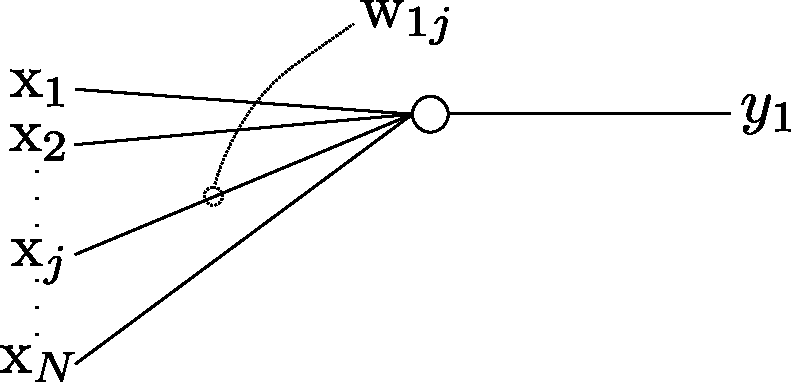
\includegraphics[width=4cm]{img/section2_fig5_a}
\captionof{figure}{A linear neuron}
\end{center}
}

\begin{itemize}
\item[] 
\only<1-3>{
Observations:\notesonly{\\}
\begin{equation}
\big\{ \vec{x}^{(\alpha)} \in \R^N \big\},\; \alpha = 1, \ldots, p,
\end{equation}
\notesonly{
\begin{equation}
\big(x_1, x_2,\ldots,x_j,\ldots,x_N\big)^\top = \vec{x} \in \R^N
\end{equation}
}

\item[] Assumption: centered data\notesonly{,
\begin{equation}\E\lbrack \vec x \rbrack = \vec 0
\end{equation}}

}

\mode<presentation>{
\only<2>{
\begin{center}

\includegraphics[width=2.5cm]{img/meme_centeronemoretime}
\end{center}
}
}
\only<3->{
\item[] Response: 
\begin{equation}
y = \sum_{j=1}^{N} w_j x_j = \vec w^{\top} \vec x \only<4>{= \lVert \vec w \rVert \, \lVert \vec x \rVert \cos \theta}
\end{equation}

\item[] We don't really have a desired output for the network.\\
\item[] However, we can interpret its response $y$.\\
}
\only<4>{

\begin{center}
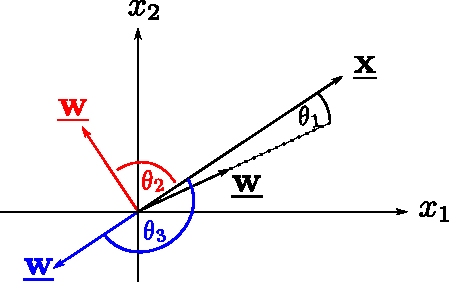
\includegraphics[width=4.5cm]{img/wxangle}
\end{center}

The inner product yields a higher value whenever $\vec x$ is ``close'' to $\vec w$.
Therefore, $y$ measures similarity between $\vec x$ and $\vec w$.
A large value of $y$ means that the network ``recognizes'' the stimulus $\vec x$.
}
\end{itemize}

\end{frame}

\newpage

\subsection{Motivation for Hebbian learnig}

\begin{frame}{\subsecname}

\begin{itemize}
\item We can use this to build associative memory (i.e. correlation learning).
\item Applicable to non-stationary data.
\item More importantly, a single linear neuron 
can organize itself such that its synaptic weights converge to a filter 
for the \slidesonly{first PC}\notesonly{\emph{first principle component}} (Oja, 1982).

\pause

\mode<presentation>{
    \begin{center}
		
\includegraphics[width=5cm]{img/meme_hebbian}
    \end{center}

}

\end{itemize}

\end{frame}

\subsection{The Hebbian learning rule}

\begin{frame}{\subsecname}
\begin{equation}
\vec w(t+1) = \vec w(t) + \underbrace{\varepsilon~y(\vec x^ {(\alpha)}; \vec w(t)) \vec x^{(\alpha)}}_{= \Delta \vec w}
\end{equation}
where $\varepsilon$ is the \emph{learning rate}.\\

\underline{The consequences of using this update rule in simulation:}\\

\begin{enumerate}
\item Divergence.\\
As $t \rightarrow \infty$ \qquad $\leadsto |\vec{w}| \rightarrow \infty$\\

\pause 

\notesonly{
\question{How does nature deal with the divergence problem?}
}

\mode<presentation>{
\only<2>{
    \begin{center}
		
\includegraphics[width=5cm]{img/meme_diverges}
    \end{center}
}
}

\pause

\item $\vec{e}_{\mathrm{w}} = \frac{\vec{w}}{|\vec{w}|}$ 
\end{enumerate}

\end{frame}

